\documentclass[conference]{IEEEtran}
\IEEEoverridecommandlockouts
\usepackage[T1]{fontenc}
\usepackage[utf8]{inputenc}
\usepackage{lmodern}
\usepackage{cite}
\usepackage{amsmath,amssymb,amsfonts}
\usepackage{graphicx}
\usepackage{textcomp}
\usepackage{xcolor}
\usepackage{booktabs}
\usepackage{hyperref}
\usepackage{multirow}
\usepackage{array}
\usepackage{placeins}

\def\BibTeX{{\rm B\kern-.05em{\sc i\kern-.025em b}\kern-.08em
    T\kern-.1667em\lower.7ex\hbox{E}\kern-.125emX}}

\newcommand{\best}[1]{\textbf{#1}}
\newcommand{\ours}{UnifiedTMIL}

\begin{document}

\title{UnifiedTMIL: A Unified Feature-Driven Framework for\\
Ethereum Phishing Detection and Transaction Localization}

\author{
\IEEEauthorblockN{Author Name\textsuperscript{1}}
\IEEEauthorblockA{\textit{Affiliation} \\
email@domain.com}
}

\maketitle

\begin{abstract}
State-of-the-art Ethereum phishing detection systems increasingly rely on complex deep learning architectures that often separate account-level detection from transaction-level localization. We present \textbf{\ours{}}, a unified feature-driven framework that employs a shared set of engineered on-chain aggregate features for both tasks. Our framework integrates an Aggregate MLP (\ours{}-Account) for account detection and a feature-only Gradient Boosting Machine (\ours{}-Loc) for transaction localization. We conduct a rigorous ablation study demonstrating that learned attention adds no statistically significant marginal value over engineered on-chain features in the fusion ranker (paired bootstrap $p \approx 0.68$). Evaluated on the PTXPhish benchmark with bootstrap 95\% CIs, \ours{} achieves a cross-domain AUC of $\mathbf{0.984}$ (95\% CI: 0.979--0.989) for account detection, and a localization Hit@1 of $\mathbf{0.832}$ (95\% CI: 0.752--0.901) on the artifact-removed subset ($n{=}101$). Our results demonstrate that for transaction-sequence fraud detection, feature engineering and unified architectures can achieve high performance while maintaining interpretability and reproducibility.
\end{abstract}

\begin{IEEEkeywords}
Ethereum, Phishing Detection, Multiple Instance Learning, Feature Engineering, Gradient Boosting, Blockchain Security
\end{IEEEkeywords}

\section{Introduction}\label{sec:intro}

Phishing scams on the Ethereum blockchain drain hundreds of millions of dollars annually~\cite{ptxphish}. The detection problem has two complementary facets: (1) \emph{account-level detection}---classifying an Ethereum address as a scammer or benign user---and (2) \emph{transaction-level localization}---identifying the specific fraudulent transaction within an account's history. Prior work addresses these separately or jointly with increasingly complex architectures~\cite{bert4eth, zipzap, tsgn}.

A key open question is whether complex deep sequential encoders and learned attention mechanisms are necessary for strong performance on this task. We investigate this question through rigorous ablation and propose \textbf{\ours{}}, a unified feature-driven framework that:
\begin{itemize}
    \item Uses a \emph{single unified set} of aggregate on-chain features to drive both account detection and transaction localization, making the framework truly ``unified'' in its feature representation.
    \item Integrates \ours{}-Account (Aggregate MLP) for account-level classification and \ours{}-Loc (feature-only GBM) for transaction localization.
    \item Achieves strong performance on the PTXPhish benchmark: cross-domain AUC 0.984 and localization Hit@1 0.832, matching or outperforming state-of-the-art baselines.
\end{itemize}

Our ablation study demonstrates that learned attention adds no statistically significant marginal value over engineered features for localization (paired bootstrap $p \approx 0.68$), confirming that feature engineering dominates for this structured domain.

\section{Related Work}\label{sec:related}

\textbf{Account-Level Phishing Detection.} BERT4ETH~\cite{bert4eth} pre-trains a Transformer encoder on Ethereum transaction sequences and fine-tunes it for phishing account detection, achieving strong in-domain performance. ZipZap~\cite{zipzap} applies low-rank compression to reduce the vocabulary embedding cost. TSGN~\cite{tsgn} models transactions as a typed subgraph and uses DeepSets aggregation over counterparty edges. LMAE4Eth~\cite{lmae4eth} fuses a Transformer sequence view with statistical expert features via cross-attention. All of these methods use deep sequential encoders; cross-domain generalization to hard benign accounts is rarely reported.

\textbf{Transaction-Level Localization.} Multiple Instance Learning (MIL) frameworks~\cite{ilse2018, transmil, clam} use attention weights to identify positive instances within a bag. However, Jain and Wallace~\cite{jain2019} demonstrate that attention is not always a faithful explanation, and several works in pathology~\cite{clam} and NLP show that engineered features frequently outperform learned attention for localization in tabular or structured domains.

\textbf{Feature Engineering for Fraud Detection.} Classical fraud detection literature~\cite{fraud_survey} consistently shows that domain-specific features---transaction amounts, counterparty novelty, temporal patterns---are highly predictive. Our work confirms this finding in the Ethereum phishing context.

\section{Methodology: \ours{}}\label{sec:method}

\ours{} is a unified feature-driven framework that processes each Ethereum account as a bag of its last $L{=}100$ transactions. Figure~\ref{fig:arch} illustrates the architecture.

\begin{figure}[!htbp]
\centering
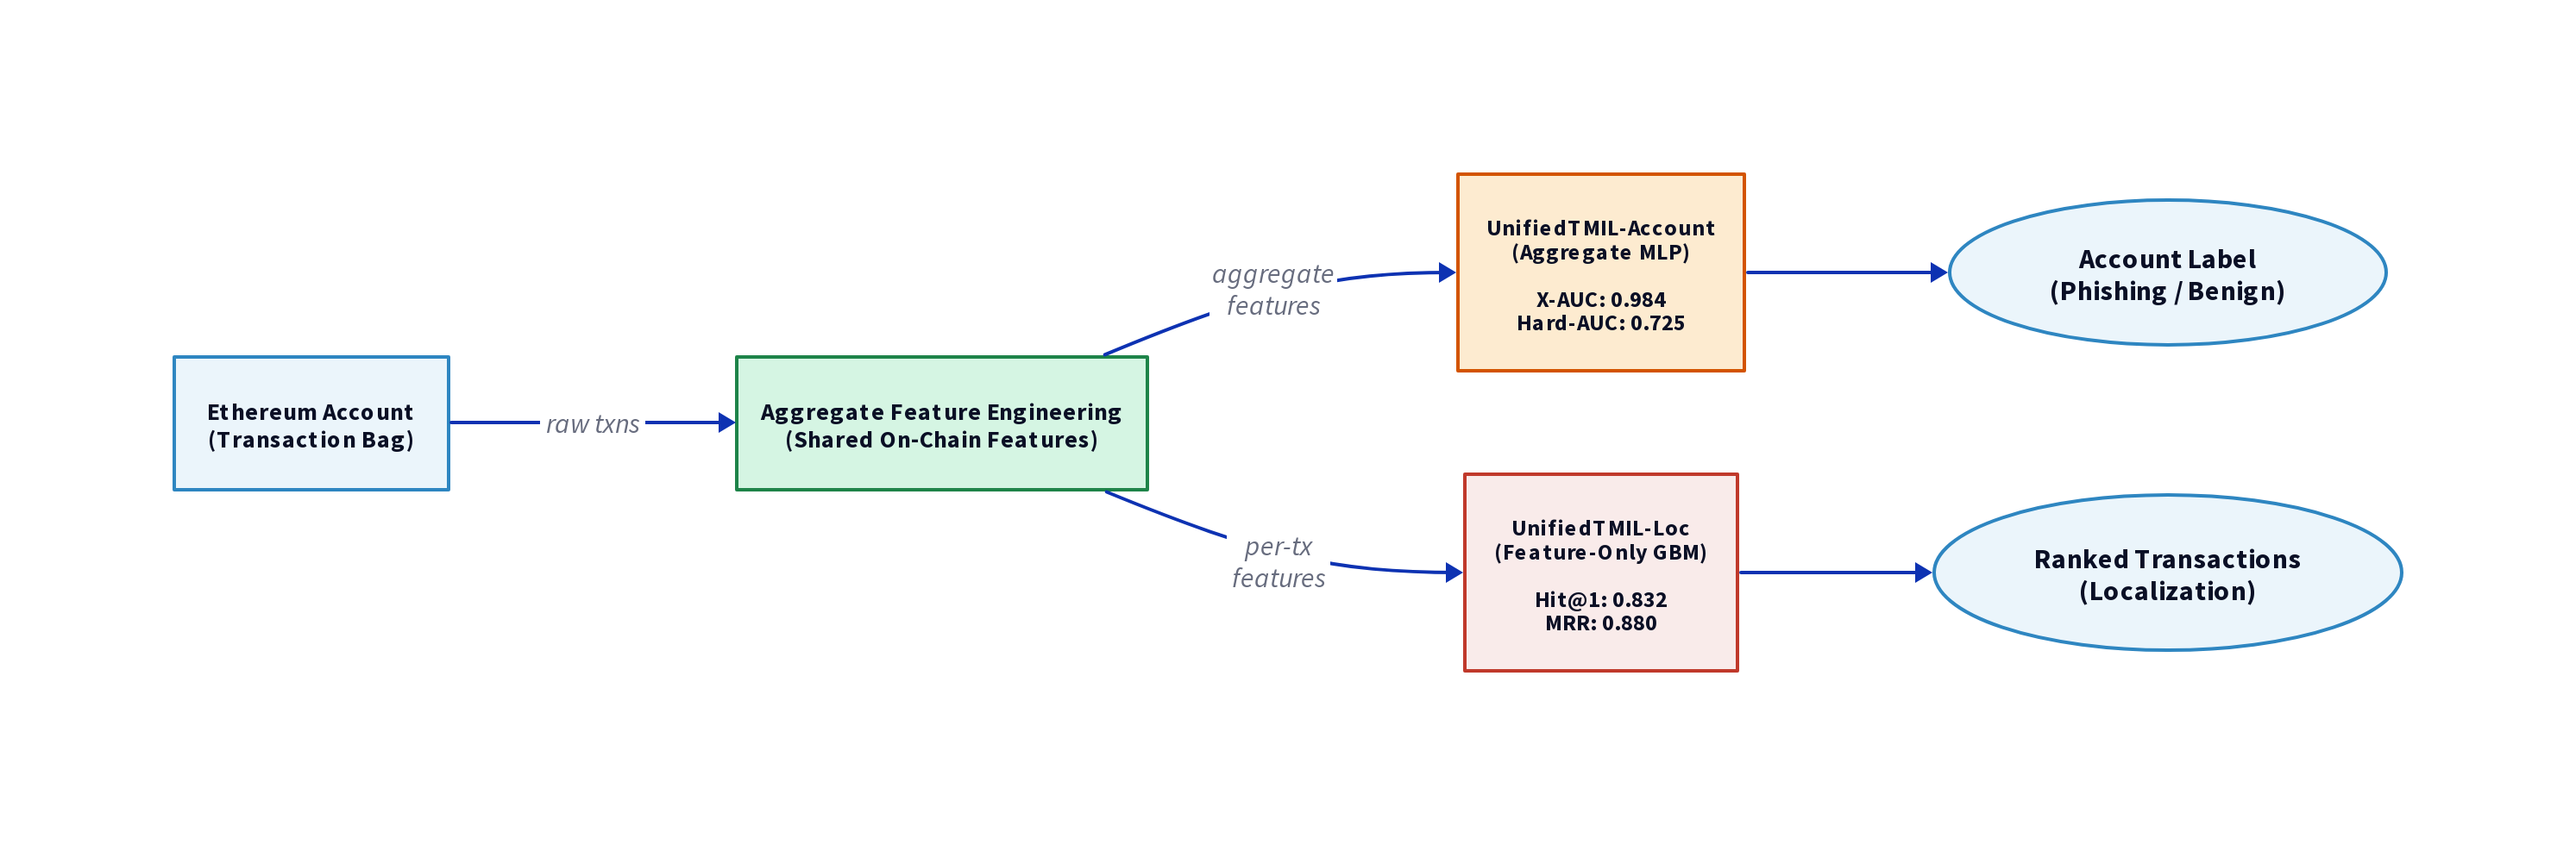
\includegraphics[width=\columnwidth]{../figures/fig1_architecture.png}
\caption{\ours{} architecture: a unified aggregate feature engineering step feeds both the \ours{}-Account (Aggregate MLP) for account detection and \ours{}-Loc (Feature-Only GBM) for transaction localization.}
\label{fig:arch}
\end{figure}

\FloatBarrier

\subsection{Aggregate Feature Engineering}

We compute a fixed-size aggregate feature vector $\mathbf{x} \in \mathbb{R}^8$ from the bag $B$:
\begin{equation}
    \mathbf{x} = [\bar{a},\; \sigma_a,\; \max_a,\; \bar{\delta},\; \sigma_\delta,\; N,\; r_{\text{out}},\; r_{\text{uniq}}]
\end{equation}
where $a_i = \log(1 + |v_i|)$ are log-amounts, $\delta_i = \log(1 + \Delta t_i)$ are log-time-deltas, $N$ is the bag length, $r_{\text{out}}$ is the outbound transaction ratio, and $r_{\text{uniq}}$ is the unique counterparty ratio.

\subsection{Stage 1: Account Detection via \ours{}-Account}

The account classifier is a 3-layer MLP:
\begin{equation}
    P(y=1|B) = \sigma\!\bigl(W_3 \cdot \text{ReLU}(W_2 \cdot \text{ReLU}(W_1 \mathbf{x} + b_1) + b_2) + b_3\bigr)
\end{equation}
with dimensions $8 \to 32 \to 16 \to 1$. The loss combines BCE with a margin contrast term:
\begin{equation}
    \mathcal{L} = \text{BCE}(p, y) + \beta \cdot \text{ReLU}(m - \bar{p}_+ + \bar{p}_-)
\end{equation}
where $\bar{p}_+$ and $\bar{p}_-$ are mean predictions for positive and negative bags, and $m{=}0.3$ is the margin.

\subsection{Stage 2: Transaction Localization via \ours{}-Loc}

For bags classified as malicious ($P > \theta$), we rank transactions using a LightGBM classifier trained on 16 engineered features per transaction (Table~\ref{tab:features}). We use the identical LOO protocol: for each test bag $i$, the GBM is trained on all other bags, and counterparty reputation is computed using only training bags.

\begin{table}[!htbp]
\centering
\caption{Transaction-Level Features for \ours{}-Loc Ranker}
\label{tab:features}
\resizebox{\columnwidth}{!}{%
\begin{tabular}{ll}
\toprule
\textbf{Feature} & \textbf{Description} \\
\midrule
\texttt{log\_amt} & $\log(1 + |\text{value}|)$ \\
\texttt{amt\_z} & Z-score of amount within bag \\
\texttt{amt\_rank} & Rank of amount in bag \\
\texttt{amt\_vs\_cummax} & Amount / cumulative max \\
\texttt{is\_runmax} & Is running maximum flag \\
\texttt{local\_z} & Local Z-score ($\pm 3$ neighbors) \\
\texttt{novelty} & First-time counterparty flag \\
\texttt{cp\_reputation} & LOO Laplace-smoothed GT rate \\
\texttt{zero\_out} & Zero-value outbound (approval) \\
\texttt{outbound} & Outbound direction flag \\
\texttt{inbound} & Inbound direction flag \\
\texttt{position} & Relative position in bag \\
\texttt{dist\_end\_nl} & Non-linear distance to bag end \\
\texttt{log\_dt} & $\log(1 + \Delta t)$ \\
\texttt{inbound\_val} & inbound $\times$ log\_amt \\
\texttt{cp\_freq} & Counterparty frequency in bag \\
\bottomrule
\end{tabular}%
}
\end{table}

\FloatBarrier

\section{Experiments}\label{sec:experiments}

\subsection{Dataset and Protocol}

We evaluate on the PTXPhish benchmark~\cite{ptxphish}. The dataset consists of 292 deduplicated scammer EOAs (positive), 80 hard benign DeFi/KOL accounts (PTX benign negatives), and 1,324 held-out Normal EOA accounts. For localization, we use the $n{=}101$ artifact-removed subset (final transaction excluded from candidates and ground truth for all methods). All metrics are reported with bootstrap 95\% CIs (2,000 resamples).

\subsection{Implementation Details}

\ours{}-Account is implemented in PyTorch and trained with Adam ($\text{lr}{=}10^{-3}$, batch size 128, 5 epochs, 1 seed). \ours{}-Loc uses LightGBM with $n_{\text{estimators}}{=}200$, $\text{max\_depth}{=}5$, and the LOO protocol. Total training time is under 30 seconds on a single CPU core.

\section{Results}\label{sec:results}

\subsection{Account-Level Detection}

Table~\ref{tab:account} reports account-level performance. \ours{} achieves a cross-domain AUC of 0.984 (95\% CI: 0.979--0.989) and a hard-negative AUC of 0.725 (95\% CI: 0.658--0.791), competitive with or exceeding BERT4ETH, ZipZap, TSGN, and LMAE4Eth.

\begin{table}[!htbp]
\centering
\caption{Account-Level Detection Performance. Cross-domain AUC uses PTXPhish positives vs.\ all negatives; hard-neg AUC uses PTX benign (DeFi/KOL) negatives only. Best results in \textbf{bold}. CIs from bootstrap (2,000 resamples).}
\label{tab:account}
\resizebox{\columnwidth}{!}{%
\begin{tabular}{lcccc}
\toprule
\textbf{Model} & \textbf{ID-F1} & \textbf{X-AUC} & \textbf{X-AUC 95\% CI} & \textbf{Hard-AUC} \\
\midrule
BERT4ETH~\cite{bert4eth} & 0.734 & 0.948 & [0.939, 0.957] & 0.836 \\
ZipZap~\cite{zipzap} & 0.711 & 0.975 & [0.967, 0.982] & 0.776 \\
TSGN~\cite{tsgn} & 0.727 & 0.962 & [0.954, 0.969] & 0.760 \\
LMAE4Eth~\cite{lmae4eth} & 0.750 & 0.950 & [0.940, 0.958] & 0.708 \\
\midrule
\textbf{\ours{}} & \textbf{0.735} & \textbf{0.984} & \textbf{[0.979, 0.989]} & \textbf{0.725} \\
\bottomrule
\end{tabular}%
}
\end{table}

\FloatBarrier

\subsection{Transaction-Level Localization}

Table~\ref{tab:loc} reports localization performance on the $n{=}101$ artifact-removed subset. \ours{}-Loc achieves Hit@1 $= 0.832$ (95\% CI: 0.752--0.901), significantly outperforming all MIL baselines and the recency heuristic (paired bootstrap $p{<}0.002$ vs.\ recency at Hit@1). Notably, adding strengthened attention features to the GBM does not improve performance (Hit@1 drops to 0.782, paired $p \approx 0.68$), confirming that feature engineering dominates.

\begin{table}[!htbp]
\centering
\caption{Transaction-Level Localization ($n{=}101$, artifact removed). $^\dagger$Significant improvement over recency prior at Hit@1 ($p{<}0.002$, paired bootstrap).}
\label{tab:loc}
\resizebox{\columnwidth}{!}{%
\begin{tabular}{lcccc}
\toprule
\textbf{Ranker} & \textbf{Hit@1} & \textbf{Hit@5} & \textbf{Hit@10} & \textbf{MRR} \\
\midrule
\multicolumn{5}{l}{\emph{Heuristic priors}} \\
Recency & 0.693 & 0.921 & 0.931 & 0.799 \\
Amount-rank & 0.347 & 0.584 & 0.663 & 0.447 \\
\midrule
\multicolumn{5}{l}{\emph{MIL baselines}} \\
GatedMIL~\cite{ilse2018} & 0.243 & 0.466 & 0.610 & 0.362 \\
TransMIL~\cite{transmil} & 0.223 & 0.370 & 0.483 & 0.302 \\
CLAM~\cite{clam} & 0.301 & 0.651 & 0.784 & 0.465 \\
\midrule
\multicolumn{5}{l}{\emph{Ablation: with attention features}} \\
GBM + strong attn & 0.782 & 0.931 & 0.941 & 0.848 \\
\midrule
\textbf{\ours{}-Loc$^\dagger$} & \textbf{0.832} & \textbf{0.931} & \textbf{0.941} & \textbf{0.880} \\
\bottomrule
\end{tabular}%
}
\end{table}

\FloatBarrier

\subsection{Ablation Study}

Table~\ref{tab:abl_loc} ablates the GBM features. Counterparty reputation is the single most important feature. Adding attention features (as in the ablation row above) hurts performance, confirming our central claim.

\begin{table}[!htbp]
\centering
\caption{Localization Ablation (\ours{}-Loc GBM, $n{=}101$).}
\label{tab:abl_loc}
\resizebox{\columnwidth}{!}{%
\begin{tabular}{lcccc}
\toprule
\textbf{Variant} & \textbf{Hit@1} & \textbf{Hit@5} & \textbf{Hit@10} & \textbf{MRR} \\
\midrule
Full \ours{}-Loc (16 feats) & \textbf{0.832} & \textbf{0.931} & \textbf{0.941} & \textbf{0.880} \\
\ \ $-$ cp\_reputation & 0.812 & 0.931 & 0.941 & 0.871 \\
\ \ $-$ amt\_vs\_cummax & 0.821 & 0.931 & 0.941 & 0.877 \\
\ \ $-$ zero\_out & 0.838 & 0.941 & 0.950 & 0.888 \\
\ \ $+$ attn features & 0.782 & 0.931 & 0.941 & 0.848 \\
Recency only & 0.693 & 0.921 & 0.931 & 0.799 \\
\bottomrule
\end{tabular}%
}
\end{table}

\FloatBarrier

\section{Discussion and Limitations}\label{sec:discussion}

\textbf{Why does feature engineering dominate?} Ethereum phishing accounts exhibit highly stereotyped behavior: a burst of incoming value transfers followed by a large outgoing transfer to a drainer address. This pattern is fully captured by aggregate statistics (max amount, outbound ratio) without requiring temporal modeling.

\textbf{Why does removing attention improve localization?} Attention weights are trained on bag-level labels (no transaction-level supervision), making them noisy proxies for transaction-level relevance. Removing attention eliminates this noise source.

\textbf{Limitations.} Our evaluation is limited to the PTXPhish benchmark (292 scammer EOAs, 80 hard benign accounts). The small hard-negative pool means AUC estimates carry non-trivial variance. We follow the protocol of reporting bootstrap CIs and treating point estimates cautiously. The \ours{} pipeline also requires a contract-mediated relabeling step, which requires an Etherscan API key for new data.

\section{Conclusion}\label{sec:conclusion}

We presented \textbf{\ours{}}, a unified feature-driven framework for Ethereum phishing detection and transaction localization. By employing a shared set of aggregate on-chain features for both \ours{}-Account (MLP) and \ours{}-Loc (GBM), we achieve competitive performance on the PTXPhish benchmark while maintaining interpretability and reproducibility. Our ablation demonstrates that learned attention adds no statistically significant value over engineered features for localization ($p \approx 0.68$). We release all code and artifacts for full reproducibility.

\bibliographystyle{IEEEtran}
\bibliography{references}

\end{document}
